\section{System Description}\label{sec:system_desc}
In Veldhoven you find the company ASML (\url{www.asml.com}).
This company makes wafer scanners.
Wafer scanners project images on silicon wafers with nano meter precision.
A scanner contains multiple chucks on which the scanner does different things.
An overview of such a wafer scanner can be found in figure~\ref{fig:system_overview}.
The scanner will move each wafer from chuck to chuck in order to project images on the wafers.
Wafers will be processed in lots in which each lot has a certain recipe.
In the following subsections facts about such a wafer scanner system are provided.

\begin{figure}[ht!]
    \centering
    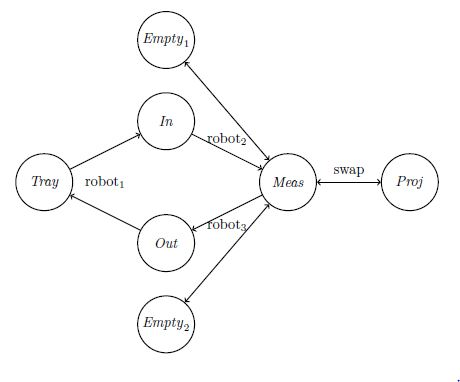
\includegraphics{img/SystemOverview.jpg}
    \caption{System overview of a wafer scanner}
    \label{fig:system_overview}
\end{figure}

\subsection{General}
\begin{itemize}
    \item The system processes a tray containing wafers.
    \item Wafers in the tray are grouped into lots.
    \item A wafer belongs to exactly one lot.
    \item A tray contains at least one lot.
    \item A lot contains at least one wafer.
    \item Each lot has a corresponding recipe.
    \item Each chuck contains at most one wafer.
    \item The system only processes complete lots.
    \item \tray contains a finite amount of lots with a finite amount of wafers.
\end{itemize}

\subsection{Recipes}
\begin{itemize}
    \item The system knows three recipes, namely \recipeOne, \recipeTwo and Recipe3.
    \item \recipeOne is that each wafer from the lot should be produced on chuck \chuckA.
    \item \recipeTwo is that each wafer from the lot should be produced on chuck \chuckB.
    \item \recipeThree is that each wafer from the lot should be produced on chuck \chuckA or chuck \chuckB.
\end{itemize}

\subsection{Chucks}
\begin{itemize}
    \item The system consists of six chucks, namely \chuckIn, \chuckOut, \chuckEmptyOne, \chuckEmptyTwo, \chuckA and \chuckB.
    \item Chuck \chuckIn stays at a fixed location.
    \item Chuck \chuckOut stays at a fixed location.
    \item Chuck \chuckEmptyOne stays at a fixed location.
    \item Chuck \chuckEmptyTwo stays at a fixed location.
    \item Chuck \chuckA and chuck \chuckB can be swapped by a robot (i.e. \robotSwap).
    \item \chuckMeas is a fixed swap location.
    \item \chuckProj is a fixed swap location.
    \item Chuck \chuckMeas is either chuck \chuckA or chuck \chuckB that is currently on position \chuckMeas.
    \item Chuck \chuckProj is either chuck \chuckA or chuck \chuckB that is currently on position \chuckProj. 
\end{itemize}

\subsection{Robots}
\begin{itemize}
    \item The system consists of four robots, namely \robotOne, \robotTwo, \robotThree, and \robotSwap.
    \item \robotOne can move wafers from \tray to chuck \chuckIn.
    \item \robotOne can move wafers from chuck \chuckOut to \tray.
    \item \robotOne can move at most one wafer.
    \item \robotTwo can move wafers from chuck \chuckIn to chuck \chuckMeas.
    \item \robotTwo can move wafers between chuck \chuckMeas and chuck \chuckEmptyOne.
    \item \robotOne can move at most one wafer.
    \item \robotThree can move wafers between chuck \chuckMeas and chuck \chuckEmptyTwo.
    \item \robotThree can move wafers from chuck \chuckMeas to chuck \chuckOut.
    \item \robotOne can move at most one wafer.
    \item \robotSwap swaps chucks between location \chuckMeas and location \chuckProj.
\end{itemize}

\subsection{Components}
\begin{itemize}
    \item The lot controller controls separate external components.
    \item There is a separate component for pre-measuring on chuck \chuckIn.
    \item There is a separate component for measuring on chuck \chuckMeas.
    \item There is a separate component for projection on chuck \chuckProj.
    \item There is a separate component for controlling \robotOne, \robotTwo, \robotThree and \robotSwap.
    \item There is a separate component for calibrating the system.
    \item Each component reports back to the lot controller when a job is completed.
\end{itemize}

\subsection{States}
\begin{itemize}
    \item \chuckIn the initial state chuck \chuckA is on location \chuckMeas.
    \item \chuckIn the initial state chuck \chuckB is on location \chuckProj.
    \item \chuckIn the initial state chuck \chuckMeas and chuck \chuckProj both contain an empty wafer and all other chucks are empty.
    \item \chuckIn the final state chuck \chuckMeas and chuck \chuckProj both contain an empty wafer and all other chucks are empty. 
\end{itemize}

\subsection{Operations}
\begin{itemize}
    \item At chuck \chuckIn a wafer is pre-measured.
    \item At chuck \chuckMeas a wafer is measured and placed with high precision.
    \item At chuck \chuckProj an image is projected onto a wafer.
    \item Calibration might be required before processing a next lot.
\end{itemize}
